\begin{frame}
    \titlepage
\end{frame}

\acrodef{CAS}{Collective Adaptive System}
\acrodef{AC}{Aggregate Computing}
\acrodef{FC}{Field Calculus}
\acrodef{XC}{Exchange Calculus}
\acrodef{GUI}{Graphical User Interface}
\acrodef{DSL}{Domain-Specific Language}
\acrodef{JVM}{Java Virtual Machine}
\acrodef{ADT}{Algebraic Data Type}
\acrodef{API}{Application Programming Interface}
\acrodef{DOT}{Dependent Object Types}
\acrodef{NPM}{Node Package Manager}

\begin{frame}
    \frametitle{Context}
    \begin{block}{Macroprogramming}
        Programming paradigm for \textbf{large-scale distributed systems} of agents aimed at expressing the \textbf{global behavior} of the system while abstracting away from the local behavior of individual components~\cite{macroprogramming-state-of-the-art}.
    \end{block}
    \begin{block}{Aggregate Computing}
        A macroprogramming technique for defining the overall behavior of a network of devices through a single program~\cite{aggregate-programming}.
        %
        \ac{AC} benefits from the \textbf{composability} of functional programming and the guarantees on emergent behavior and properties provided by its formalization: the \textbf{\ac{FC}}~\cite{fc}.
    \end{block}
\end{frame}

\begin{frame}
    \frametitle{State of the Art}
    \begin{blockitems}{ScaFi: an Aggregate Programming framework written in Scala 2}
        \item \textbf{Internal \ac{DSL}}: ScaFi offers an internal domain-specific language for defining aggregate programs~\cite{scafi}
        \item \textbf{Scala 2}: the host language for ScaFi is Scala 2, natively targeting the \ac{JVM}~\cite{scafi-thesis}
        \item \textbf{Based on \ac{FC}}: ScaFi's construct syntax and semantics are based on the Field Calculus formal language
        \item \textbf{Runtime}: the framework offers a runtime environment for executing aggregate programs on a network of devices based on \textit{Akka}
        \item \textbf{Simulation}: ScaFi provides a simulation environment for testing aggregate programs, with \acp{GUI}, as well as integration with the \textbf{Alchemist} simulator~\cite{alchemist,scafi-with-alchemist}
        \item \textbf{Multiplatform}: the core and simulator of ScaFi are compiled into JavaScript and delivered though \ac{NPM}
    \end{blockitems}
\end{frame}

\begin{frame}
    \frametitle{Background and Motivation}
    \begin{blockitems}{The \ac{XC}}
        \item A \textbf{new formal language} for aggregate programming~\cite{xc}
        \item \textbf{More expressive} than \ac{FC}, from which it takes inspiration
        \item Based on a \textbf{single communication primitive}: \texttt{exchange}, thus simplifying formal reasoning, while \ac{FC} has three main primitives (\textit{rep}, \textit{nbr}, and \textit{share})
        \item \ac{FC} core constructs can be implemented in \ac{XC}, thus \ac{XC} inherits the same results found in literature for \ac{FC}
    \end{blockitems}
\end{frame}

\begin{frame}
    \frametitle{Background and Motivation}
    \begin{blockitems}{Scala 3}
        \item A new major version of the Scala language, with \textbf{improved syntax} and \textbf{new features}, such as \textit{extension methods}, improved \textit{\acp{ADT}}, indentation-based syntax, \textit{path-dependent types}, \textit{abstract type members}, \textit{abstract given instances} and more
        \item Offers experimental features such as \textit{safe initialization}, \textit{explicit nulls}, and \textit{multiversal equality}, all employed in this work
        \item Promotes the migration of existing Scala 2 codebases to Scala 3
        \item Featuring cross-compilation to Scala 2, JavaScript, and native code
        \item Compiled with the new \textit{Dotty} compiler, based on the formal \ac{DOT} calculus
    \end{blockitems}
\end{frame}

\begin{frame}
    \frametitle{Key Users}
    \begin{itemize}
        \item \textbf{End users}: who uses \this to write aggregate programs
        \item \textbf{Library developers}: who takes care of extending the standard library of \this with new features, constructs, and syntax
        \item \textbf{Researchers}: who experiments with the formal calculus foundation od \this and could benefit from reusing existing libraries
    \end{itemize}
\end{frame}

\begin{frame}
    \frametitle{Requirements}
    \begin{itemize}
        \item Redesign and implement a new \ac{DSL} \ac{API} for the \texttt{core} module, using Scala 3 features
        \item Use \ac{XC} as the formal foundation for the new \ac{DSL} implementation
        \item Support the new \ac{DSL} with a pure Scala 3 simulator, avoiding third-party dependencies
        \item Write meaningful acceptance tests for validating the entire suite
        \item Optionally, integrate the \texttt{core} with the Alchemist simulator
    \end{itemize}
\end{frame}

\begin{frame}
    \frametitle{\ac{DSL} Design}
    Four prototypes have been implemented and evaluated with the \textit{key users} to collect feedback and decide the final design.

    \textbf{Final version of the \ac{DSL}:}
    \begin{itemize}
        \item \texttt{AggregateFoundation} as the base trait for all calculi syntaxes
        \item \ac{XC} implemented both as a syntax trait and as a semantics foundation
        \item The entire \ac{DSL} library is generic in the calculus it supports, only cares about available operations and syntax
        \item Actual implementation of the semantics is left to runtime providers, albeit \this offers a default implementation of the \ac{XC} semantics
    \end{itemize}
\end{frame}

\begin{frame}
    \frametitle{Implementation Milestones}
    \begin{itemize}
        \item \textbf{Engine} module: round-based aggregate program execution
        \item \textbf{Simulator} module: pure Scala 3, in-memory, without \ac{GUI}
        \item \textbf{Alchemist} module: Integration with the Alchemist simulator, for running aggregate programs in a more realistic environment, with customizable \ac{GUI}
        \item \textbf{Tests}: both unit tests for components and \textbf{acceptance tests} for simulated networks
        \item \textbf{Code Quality}: enforced by static analysis tools, pedantic compilation flags, and continuous integration
        \item \textbf{Cross-compilation}: pure Scala 3, targets the \ac{JVM}, JavaScript, and native code
    \end{itemize}
\end{frame}

\begin{frame}
    \frametitle{Simulation visualization with Alchemist}
    \begin{figure}
        \label{fig:alchemist-demo}
        \centering
        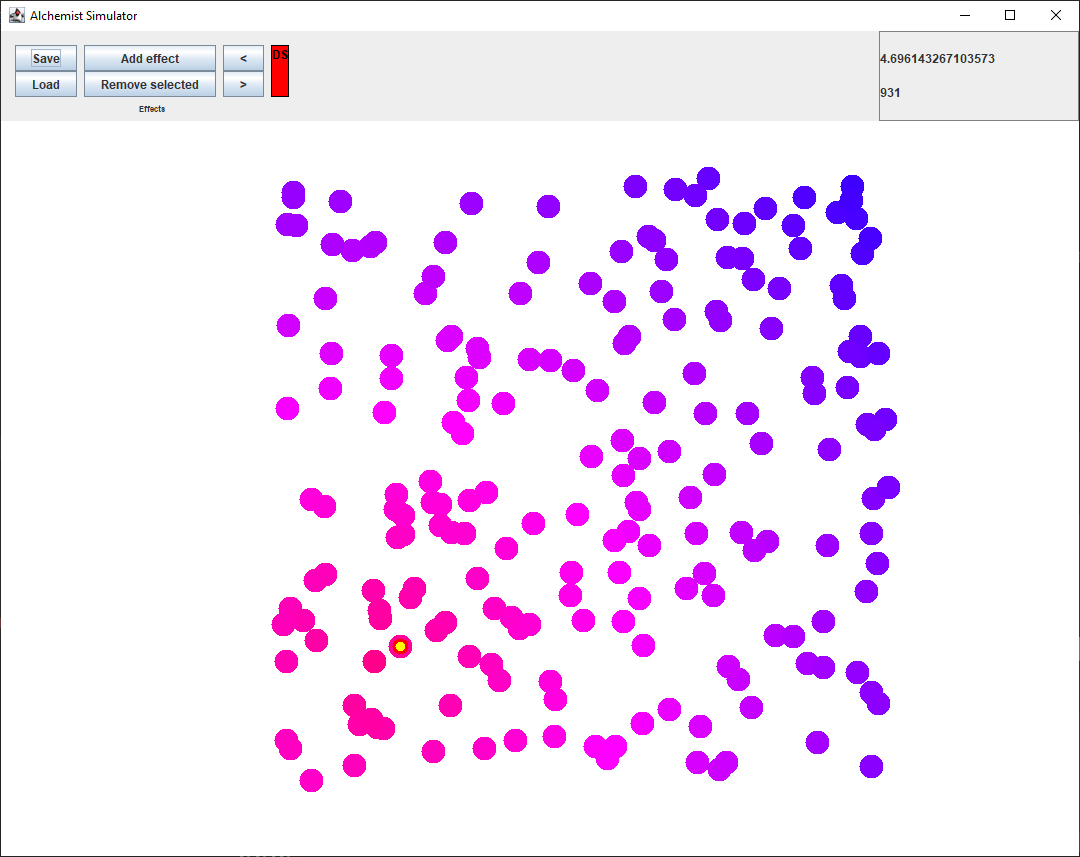
\includegraphics[width=0.66\textwidth]{figures/alchemist-demo.png}
        \caption{A screenshot of the Alchemist simulator, showing a network of devices running an aggregate program that computes a gradient from a source.}
    \end{figure}
\end{frame}

% \begin{frame}
%     \frametitle{Comparison with the State of the Art: FCPP}
%     \begin{exampleblock}{FCPP~\cite{fcpp}}
%         \lstinputlisting[xleftmargin=10pt, language=C++, caption={Gradient distance from a source in FCPP.}, label={lst:gradient-distance-fcpp}]{listings/fcpp-gradient-distance.cpp}
%     \end{exampleblock}
% \end{frame}

% \begin{frame}
%     \frametitle{Comparison with the State of the Art: Protelis}
%     \begin{exampleblock}{Protelis~\cite{protelis}}
%         \lstinputlisting[xleftmargin=10pt, language=Protelis, caption={Gradient distance from a source in Protelis.}, label={lst:gradient-distance-protelis}]{listings/protelis-gradient-distance.pt}
%     \end{exampleblock}
% \end{frame}

\begin{frame}
    \frametitle{Comparison with the State of the Art: ScaFi}
    \begin{exampleblock}{ScaFi}
        \lstinputlisting[xleftmargin=10pt, language=Scala, caption={Gradient distance from a source in ScaFi.}, label={lst:gradient-distance-scafi}]{listings/scafi-gradient-distance.scala}
    \end{exampleblock}
\end{frame}

% \begin{frame}
%     \frametitle{Comparison with State of the Art: \ac{XC}}
%     \begin{exampleblock}{\ac{XC}}
%         \lstinputlisting[xleftmargin=10pt, language=XC,label={lst:xc-program}, caption={Gradient distance from a source written with the XC language.}]{listings/xc-gradient-distance.xc}
%     \end{exampleblock}
% \end{frame}

% \begin{frame}
%     \frametitle{Comparison with the State of the Art: \this}
%     \begin{exampleblock}{\this - GradientLibrary: distanceEstimate}
%         \lstinputlisting[xleftmargin=10pt, language=Scala, caption={\texttt{distanceEstimate} implementation in \this.}, label={lst:distance-estimate}]{listings/distance-estimate.scala}
%     \end{exampleblock}
% \end{frame}

\begin{frame}
    \frametitle{Comparison with the State of the Art: \this}
    \begin{exampleblock}{\this - GradientLibrary: distanceTo}
        \lstinputlisting[xleftmargin=10pt, language=Scala, caption={\texttt{distanceTo} implementation in \this.}, label={lst:distance-to}]{listings/distance-to.scala}
    \end{exampleblock}
\end{frame}

\begin{frame}
    \frametitle{Experiments with Scala 3 and the \ac{DSL}}
    \begin{itemize}
        \item Implementation of a \texttt{FoldhoodLibrary} that provides a \textit{foldhood} \ac{API} similar to the one in ScaFi, proving the expressiveness of the \this \ac{DSL}
        \item Implementation of a series of constraints for aggregate programming correctness that can be statically checked by the Scala 3 compiler, without using macros or metaprogramming, only relying on context bounds and given instances.
    \end{itemize}
\end{frame}

\begin{frame}
    \frametitle{Conclusions}
    \begin{itemize}
        \item Successful redesign and implementation of a new \ac{DSL} for the \texttt{core} module of \this, using advanced programming patterns and Scala 3 features, serving as the foundation for future developments in the \ac{AC} field
        \item Satisfaction of all the requirements, including optional ones, such as the integration with the Alchemist simulator
        \item Code quality and maintainability enforced with static analysis, continuous integration, and evaluated with peer reviews
    \end{itemize}
    \begin{blockitems}{Future Work}
        \item Performance optimization: the current implementation only focuses on correctness, reusability, and readability
        \item Improvement of the simulator
        \item Support real-world deployment use cases with the equivalent of the \texttt{distributed} module in ScaFi
        \item Add more standard libraries and acceptance tests
    \end{blockitems}
\end{frame}

\begin{frame}
    \frametitle{Acknowledgments}
    \begin{blockitems}{Supervisors}
        \item Prof. Mirko Viroli
        \item Dr. Gianluca Aguzzi
        \item Dr. Roberto Casadei
    \end{blockitems}
    \begin{block}{Others}
        Thanks to all the people who contributed to the development of \this, including the authors of the original ScaFi framework, the Alchemist simulator, the \ac{XC} formal language, and the community of Scala 3 developers.

        Thanks to my family and friends for their support and patience.

        \textit{Thank you for your attention.}
    \end{block}
\end{frame}
